\documentclass[11pt,a4paper]{article}

\usepackage[utf8]{inputenc}
\usepackage{amsmath,amssymb}
\usepackage{graphicx}
\usepackage{subcaption}
\usepackage{float} % only needed if you use [H]
\usepackage{hyperref}
\usepackage{geometry}
\usepackage{setspace}
\usepackage{booktabs}
\usepackage{tabularx}
\usepackage{cancel}
\geometry{a4paper, margin=2.5cm}
\onehalfspacing

\title{A Phenomenological Study of Early--Late Azimuthal Asymmetries of the Muon Density with the UMD}
\author{Lautaro Silva Pizzi, Juan Manuel Figueira and Federico S\'anchez \\ Pierre Auger Observatory}
\date{August 2026}

\begin{document}

\maketitle

\begin{abstract}
We revisit the phenomenology of early--late azimuthal asymmetries in the muon density of extensive air showers and, for the first time, extend the analysis to the Underground Muon Detector (UMD) of the AMIGA enhancement of the Pierre Auger Observatory. Using a set of \texttt{CORSIKA}/\texttt{Offline} simulations processed with \texttt{Sibyll\,2.3e} in the energy interval $\log_{10}(E/\mathrm{eV})\in[17.5,18.0]$, we characterise the competition between the three dominant physical mechanisms that shape the azimuthal modulation: atmospheric attenuation, the geometric effect, and the kinematic projection of muons. By combining a controlled Dense Ring topology, which decouples azimuthal from radial effects, with the continuous radial coverage of the SD-750 array, we show that the Surface Detector (SD) total signal undergoes a pronounced sign inversion of the first-harmonic amplitude $A_1$ at large core distances ($r\gtrsim 750$~m), driven by the abundant, highly divergent low-energy muon population. In contrast, the $\gtrsim 540~\mathrm{g/cm^2}$ soil overburden of the UMD imposes an effective kinematic threshold $E_\mu\gtrsim 1~\mathrm{GeV}/\cos\theta$ that suppresses this divergent population, collapsing the kinematic divergence contribution to the asymmetry to a negligible level. As a result, the UMD preserves a positive, monotonic, attenuation-dominated asymmetry throughout the accessible parameter space, establishing it as a phenomenologically cleaner tracer of the longitudinal development of the cascade.
\end{abstract}

\section{Introduction}
\label{sec:intro}

The azimuthal asymmetry of the particle density footprint at ground level has long been recognised as a sensitive probe of the longitudinal development of extensive air showers (EAS). Early phenomenological studies by Pryke \cite{Pryke1998} and by Billoir and collaborators \cite{Billoir2002, GAP2000_017}, later extended by Dembinski et al. \cite{GAP2007_124}, established the analytical framework in which the ground densities of inclined showers are parametrised by a first-order harmonic modulation and identified attenuation and geometric projection as its two leading sources. In this framework, the particle density $S$ in the shower plane is expressed as:

\begin{equation}
    S(r, \phi) = \langle S(r)\rangle \big[ 1 + A_1(r, \theta) \cos \phi \big] ,
    \label{eq:harmonic_fit}
\end{equation}
%
where $\langle S(r)\rangle$ is the azimuthally averaged density at radial distance $r$, and $A_1(r, \theta)$ is the amplitude of the early–late modulation. Following this convention, $A_1 > 0$ corresponds to a density peak in the early region, while $A_1 < 0$ corresponds to a density peak in the late region. The $\sin \phi$ term is omitted, as it averages to zero for isotropic arrival directions, and the expansion is truncated at first order because higher-order harmonics remain small in the targeted parameter space. 

More recently, and in the context of the AugerPrime upgrade \cite{AugerPrime2016}, Bradfield \cite{BradfieldThesis} performed a comprehensive systematic study of asymmetries using both the Water Cherenkov Detector (WCD) and the Surface Scintillator Detectors (SSD), confirming the utility of azimuthal modulations as a mass-composition observable. 

All of these analyses share a common limitation: the Surface Detector (SD) measures a signal combining the electromagnetic (EM) and muonic components of the cascade. As a consequence, SD-based asymmetry observables exhibit non-trivial features, including a suppression of the amplitude for deeply developing showers and an outright sign inversion of $A_1$ at large radial distances \cite{BradfieldThesis, Luce_ICRC2021}. This far-core inversion is driven by a third phenomenon, the kinematic divergence of low-energy muons, which heavily competes against the other two. Disentangling these three competing effects requires a detector that is intrinsically sensitive to the muonic component only.

The purpose of this work is therefore twofold. First, we extend the asymmetry analysis pioneered on the SD to the UMD, a study not previously reported. The UMD, part of the AMIGA extension~\cite{Botti2019, auger2020umd_infill}, consists of segmented plastic scintillators buried 2.3-m underground. The resulting approximately $\sim 540~\mathrm{g/cm^2}$ soil overburden imposes an effective muon energy threshold of $E_\mu \gtrsim 1 ~\mathrm{GeV}/\cos\theta$, acting as a kinematic filter of incoming muons whose selectivity itself depends on zenith angle, and it suppresses the EM component to a negligible level. Second, by exploiting a controlled Dense Ring topology together with the continuous radial spectrum of the SD-750 array, we dissect the competing physical mechanisms that govern the azimuthal modulation and provide a quantitative interpretation of the SD muon inversion reported in~\cite{Luce_ICRC2021} in terms of the Caz\'on kinematic model~\cite{Cazon2012}.

We restrict our analysis to proton and iron initiated showers in the energy range $\log_{10}(E/\mathrm{eV}) \in [17.5, 18.0]$ simulated over the zenith range $\theta \in [0^\circ, 65^\circ]$. The note is structured as follows. In Section~\ref{sec:physics}, we lay out the theoretical framework and the physical sources of azimuthal asymmetry. In Section~\ref{sec:methodology}, we detail the Monte Carlo (MC) production parameters and the evaluation topologies. Section~\ref{sec:results} presents the phenomenological results, contrasting the intrinsic asymmetry of the UMD with the convolved SD signal, and Section~\ref{sec:conclusions} summarises our findings and their implications for future mass-composition studies.

\section{Physical Sources of Azimuthal Asymmetries}
\label{sec:physics}

Before quantifying the asymmetry, it is convenient to distinguish the two reference frames involved in the analysis: the ground plane (topographic frame) and the shower plane, defined as the plane orthogonal to the shower axis. The radial distance to the core $r$ and the azimuthal angle $\phi$ are defined strictly in the shower plane throughout this work, as illustrated in Figure~\ref{fig:shower_plane}.

For a vertical shower ($\theta = 0^{\circ}$), the two frames coincide and the particle density is, up to shower-to-shower fluctuations and small deflections induced by the geomagnetic field, symmetric around the shower axis. Consequently, iso-density contours at ground level are circles centred on the core. The core is defined as the position where the axis along which the shower evolves intersects with the ground. Vertical showers are therefore taken as the reference configuration with no azimuthal asymmetry.

\begin{figure}[h]
\centering
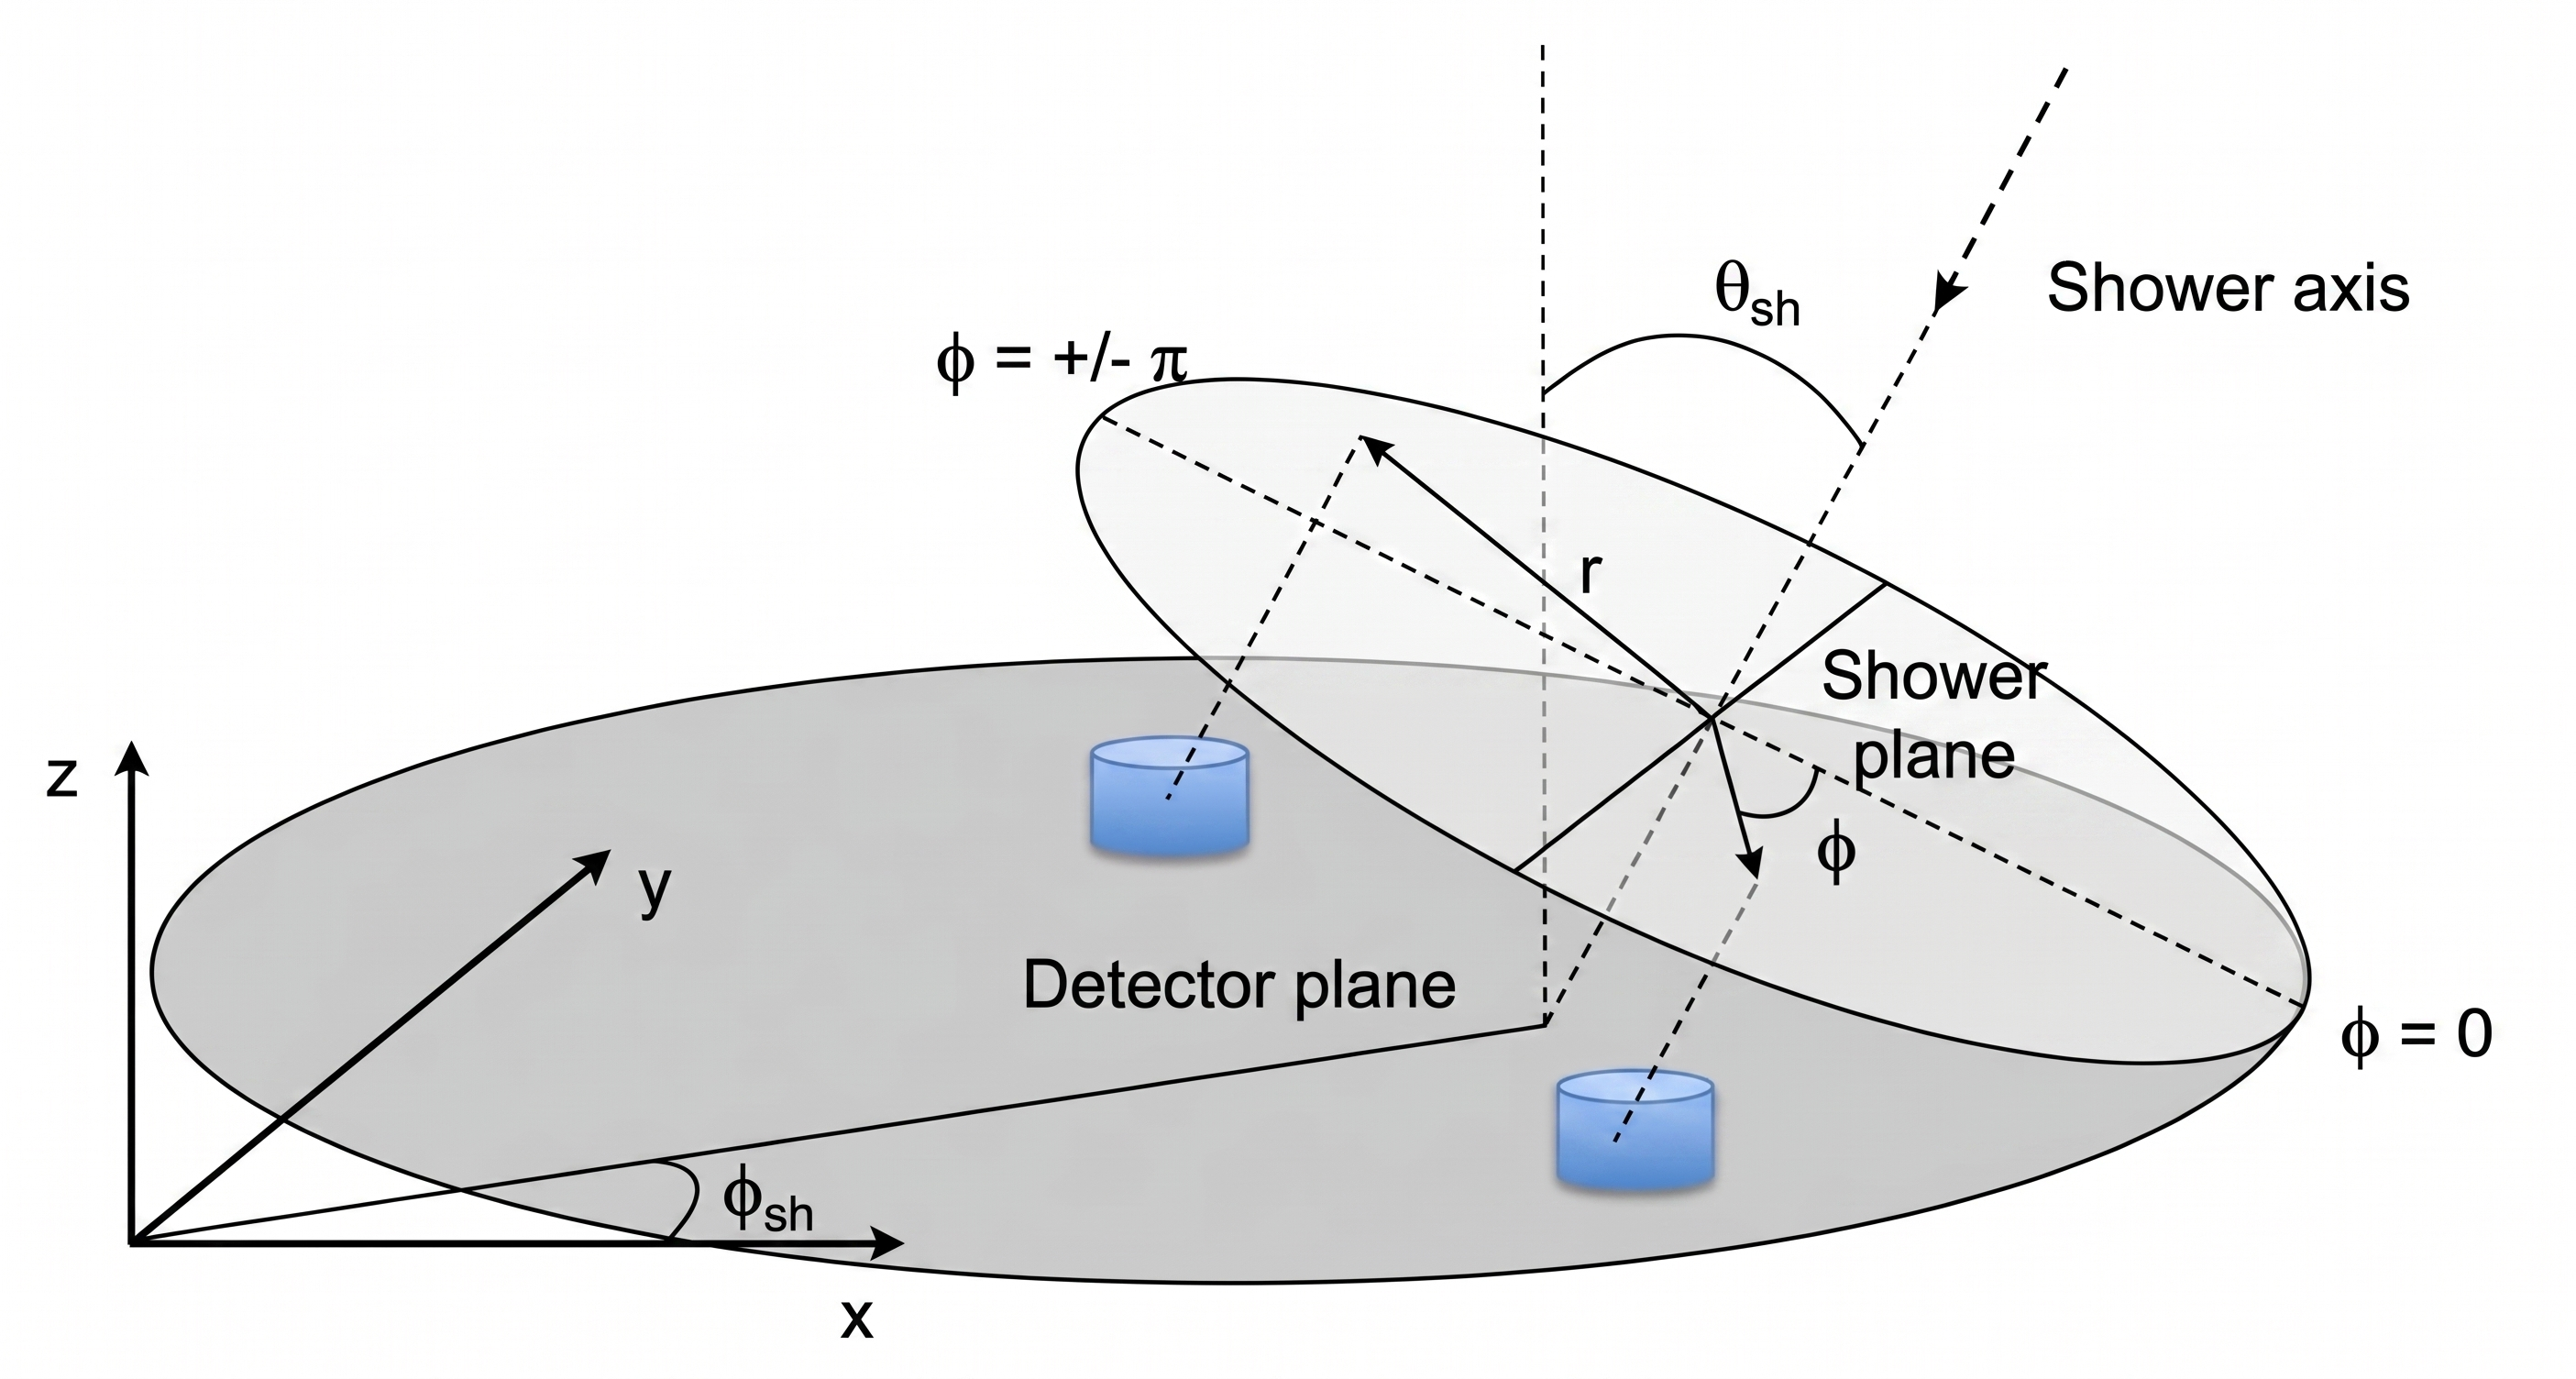
\includegraphics[width=1\textwidth]{esquema_lluvia.jpeg}
\caption{Geometric schematic of an EAS. Detector positions on the ground plane are projected onto the shower plane to define the intrinsic coordinates $r$ and $\phi$.}
\label{fig:shower_plane}
\end{figure}

For an inclined primary ($\theta > 0^{\circ}$), the shower plane is tilted with respect to the ground, breaking the circular symmetry from the point of view of an observer on the array (see Figure \ref{fig:shower_plane}). Two azimuthal regions are conventionally defined for detectors located at the same radial distance $r$ in the shower plane:

\begin{itemize}
\item \textbf{Early region ($\phi \approx 0^{\circ}$):} the section of the shower front closest to the ground, where particles impact the array first and traverse the shortest atmospheric slant depth.
\item \textbf{Late region ($\phi \approx \pm 180^{\circ}$):} the diametrically opposite section, i.e., the section of the shower front which remains elevated when the early side has already hit the ground. Particles here propagate through a larger atmospheric depth before detection.
\end{itemize}

The resulting azimuthal modulation reflects the superposition of two competing physical mechanisms, which we now discuss in turn.

\subsection{Mechanisms Driving the Early Excess}
\label{subsec:early_excess}

Two independent physical phenomena act to increase the particle density in the early region relative to the late region, driving a positive asymmetry.

\subsubsection{Atmospheric Attenuation}

Because the late region of an inclined shower is more elevated relative to the ground than the early region, particles travelling towards $\phi \approx \pm 180^{\circ}$ traverse a larger atmospheric depth than those arriving at $\phi \approx 0^{\circ}$. As the cascade develops and its particle content is progressively absorbed, this asymmetric slant depth translates into a density excess in the early direction and a deficit in the late direction~\cite{Pryke1998,dova2003,BradfieldThesis}. While muons are considerably more penetrating than the EM component, at the energies relevant for the UMD, both energy losses and muon decay in flight produce a sizeable positive contribution to the early-late asymmetry.

\subsubsection{Geometrical Flux Projection}

As originally noted by Billoir \cite{GAP2000_017}, an event that is perfectly symmetric in the shower reference frame will appear asymmetric when projected onto the ground plane. Particles hitting the ground in the early region intersect the ground plane more perpendicularly than those in the late region (as illustrated by $\theta_{late} < \theta_{early}$ in Figure 2), thereby presenting a larger cross-sectional flux per unit area. Bertou and Billoir parametrized the angular modulation of this specific projection as 

\begin{equation}
    \mathcal{A}_{geo}(r, \phi, \theta) = A_{geo}(r, \theta) \cos \phi
    \label{eq:geometric_effect_full}
\end{equation}
%
where the radial dependant amplitude is defined as \cite{GAP2000_017}:

\begin{equation}
    A_{geo}(r, \theta) = \left\langle \frac{p_t(r)}{-p_z(r)} \right\rangle \tan \theta
    \label{eq:geometric_effect}
\end{equation}
%
where $p_t$ and $p_z$ are the transverse and longitudinal momentum components, respectively. We adopt the convention that $p_z < 0$ for downward-going particles. Therefore, the denominator $-p_z$ is positive. Since $p_t$ and $\tan\theta$ are also positive, the amplitude $A_{geo}$ is strictly positive, yielding a local maximum in the early region ($\phi = 0^\circ$). Thus, the geometric flux projection acts additively with atmospheric attenuation to drive a positive asymmetry.

While Billoir's geometric projection ($\mathcal{A}_{geo}$) correctly predicts an early excess by treating the cascade locally as a plane wave, it fails to capture the global divergence of the particles from their production point high in the atmosphere. To explain the late excess observed in the far-core region, we must evaluate the kinematic divergence of the emission angles, as modelled by Cazón and Luce \cite{Cazon2012, Luce_ICRC2021}.

\subsection{Kinematic Divergence: Driving the Late Excess}
\label{subsec:divergence}

Competing directly against the early excess is a purely kinematic mechanism arising from the angular distribution of the particles, which generates a severe density excess in the late region. 

To understand this phenomenon, it is necessary to analyse the kinematics of muon production. Following the transport model of Cazón et al.~\cite{Cazon2012}, muons are produced in the hadronic cascade at a distance $D$ along the shower axis from the decay of charged pions and kaons. During this process, they inherit a longitudinal momentum $p_z$ and a transverse momentum $p_t$, which causes the muon to be emitted with a polar divergence angle $\alpha$ relative to the shower axis obeying

\begin{equation}
    \sin \alpha \simeq \frac{c p_t}{E} \simeq \frac{p_t}{|p_z|},
    \label{eq:cazon_alpha}
\end{equation}
%
where the last equality holds in the ultra-relativistic limit $|p_z| \gg m_\mu c$.

As the particle beam propagates toward the ground, the muon density $S$ recorded by a detector is dictated by two competing factors: the muon expansion of the beam and the hadronic emission spectrum. First, the spatial density falls off with the square of the geometric distance travelled ($d$). Because the differential transverse area grows spherically as $dA = d^2 d\Omega$, the density is inversely proportional to $d^2$ and directly proportional to the number of particles emitted per solid angle:

\begin{equation}
    S \propto \frac{1}{d^2} \frac{dN}{d\Omega}.
\end{equation}

Second, the number of particles emitted per unit of solid angle, $\frac{dN}{d\Omega}$, decays abruptly as more extreme angles are demanded. As modelled by Cazón et al.~\cite{Cazon2012}, the transverse momentum ($p_t$) distribution of secondary particles is parametrized with a linear factor and an exponential tail as $dN/dp_t \propto p_t \exp(-p_t/Q)$, where $Q$ is an empirical scale parameter representing the characteristic transverse momentum exchange of the interaction.

To evaluate the ground density, this momentum distribution needs to get transformed into an angular emission distribution. By defining the differential solid angle and applying the exact kinematic relation $p_t = p \sin\alpha$:

\begin{equation}
    d\Omega \propto \sin\alpha \, d\alpha \quad \& \quad dp_t = p \cos\alpha \, d\alpha.
    \nonumber
\end{equation}

By substituting $d\alpha$, one can express the solid angle element directly in terms of the transverse momentum differential:

\begin{equation}
    d\Omega \propto \sin(\alpha)\left(\frac{dp_t}{p\cos(\alpha)}\right) \overset{\times \frac{p}{p}}{=} \frac{p \sin\alpha}{p^2 \cos\alpha} \, dp_t = \frac{p_t}{p^2 \cos\alpha} \, dp_t.
\end{equation}

Then applying the chain rule to the momentum distribution. The linear $p_t$ factor exactly cancels out, leaving an angular distribution driven solely by the cosine projection and the exponential tail:

\begin{equation}
    \frac{dN}{d\Omega} = \frac{dN}{dp_t} \frac{dp_t}{d\Omega} \propto \Big( \cancel{p_t} \exp(-p_t/Q) \Big) \left( \frac{p^2 \cos\alpha}{\cancel{p_t}} \right) \propto \cos(\alpha) \exp(-p_t/Q).
\end{equation}

Finally one can express the transverse momentum as a function of the emission angle and energy, $p_t \simeq \frac{\sin(\alpha) E}{c}$ from Eq. \eqref{eq:cazon_alpha}. Substituting this relation into the angular emission spectrum and combining it with the spatial expansion yields the fundamental scaling for the ground muon density:

\begin{equation}
    S(d, \alpha) \propto \frac{1}{d^2} \cos(\alpha) \exp\left(-\frac{\sin(\alpha) E}{cQ}\right).
    \label{eq:kinematic_divergence}
\end{equation}

In an inclined shower, reaching an identical radial distance $r$ in the shower plane requires particles to travel different distances to the ground depending on their azimuth. For a production distance $D$, the distance to the ground is $d(\phi) \approx D - r \sin\theta \cos\phi$. Consequently, the early region ($d_{early} \approx D - r \sin\theta$) is physically closer than the late region ($d_{late} \approx D + r \sin\theta$). 

To reach the identical radius $r$, the emission angle required to impact the late region must be strictly smaller ($\alpha_{late} < \alpha_{early}$). This geometric compression is illustrated in Figure \ref{fig:divergence_angles}.

\begin{figure}[h]
    \centering
    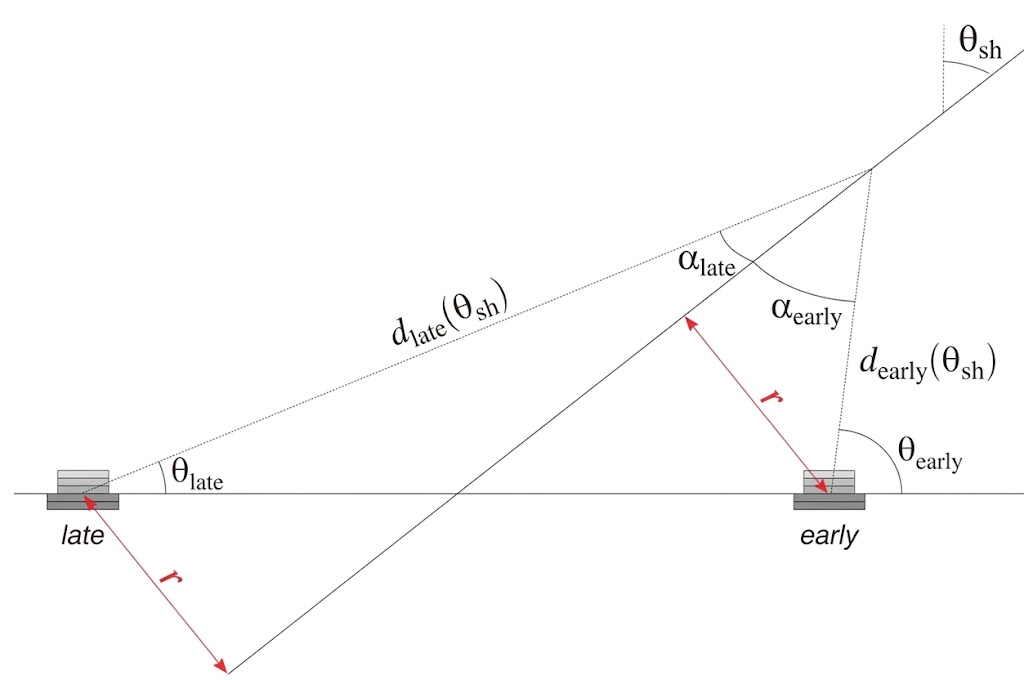
\includegraphics[width=1\textwidth]{efecto_geo_luce_icrc2021.png} 
    \caption{Geometric schematic of particle dispersion. Due to the shower inclination, reaching the same radial distance $r$ in the late region requires an emission angle $\alpha_{late}$ that is significantly smaller than the one required for the early region $\alpha_{early}$. It is also shown that the angle of arrival to the ground is more perpendicular in the early region than the late region ($90^\circ \sim \theta_{early} > \theta_{late}$) \cite{Luce_ICRC2021}.}
    \label{fig:divergence_angles}
\end{figure}

By taking the ratio of the density in the late region to the early region, we can evaluate the severe competition between the spatial expansion and the hadronic emission spectrum:

\begin{equation}
   \frac{S_{late}}{S_{early}} \approx \left( \frac{d_{early}}{d_{late}} \right)^2 \left( \frac{\cos \alpha_{late}}{\cos \alpha_{early}} \right) \exp\left( \frac{(\sin \alpha_{early} - \sin \alpha_{late}) E}{cQ} \right).
\end{equation}

%FALTAN COMENTARIOS ACA


The physical interpretation of this ratio exposes why the late region develops an excess of particles. Because the late region is further away ($d_{late} > d_{early}$), the squared distance ratio is strictly less than 1. If this spatial reduction were the only active effect, the late region would exhibit a lower density.

However, because reaching the late region demands a more collimated trajectory ($\alpha_{late} < \alpha_{early}$), we find that $\cos(\alpha_{late}) > \cos(\alpha_{early})$. Thus, the phase-space ratio ($\cos\alpha_{late}/\cos\alpha_{early}$) is strictly greater than 1, acting as an additional statistical gain for the late region. Furthermore, the subtraction $\sin(\alpha_{early}) - \sin(\alpha_{late})$ yields a positive value, forcing the exponential term to also be strictly greater than 1. 

In the dynamics of the cascade, these two gains occur because hadronic collisions overwhelmingly produce particles that travel nearly straight forward along the shower axis (small emission angles), rather than scattering widely. Because the number of produced particles increases exponentially as the emission angle decreases, this massive statistical advantage easily overcomes the $1/d^2$ density loss caused by the longer travel distance. Empirically, the fact that this exponential gain dominates the spatial expansion is confirmed by the severe negative asymmetry measured by surface detectors at large radial distances. As a result, a strong artificial density excess is projected onto the late region ($\phi = \pm 180^\circ$).

These effects motivate the phenomenological distinction of two muon populations sampled at a given radius:

\begin{itemize}
    \item \textbf{Population A (High Energy):} In hadronic collisions, the transverse momentum $p_t$ acquired by secondary particles is strictly bounded by interaction kinematics. Because the total momentum of the particle is the vector sum of its longitudinal and transverse components ($p^2 = p_z^2 + p_t^2$), a muon can only achieve a high total energy if its longitudinal momentum $p_z$ is exceptionally large. Consequently, for high-energy muons, the longitudinal component vastly outweighs the bounded transverse component ($|p_z| \gg p_t$). As a result, their divergence angle $\alpha$ is very small, and their trajectories are highly collimated. The exponential advantage vanishes, and these particles maintain the positive attenuation asymmetry.
    
    \item \textbf{Population B (Low Energy):} Conversely, for muons with low total energy, the longitudinal momentum drops to values small enough to be comparable to the bounded transverse momentum ($|p_z| \sim p_t$). This specific kinematic regime forces large divergence angles. It is this wide angular dispersion that triggers the exponential gain and projects the severe late excess onto the ground.
\end{itemize}

Because the energy spectrum of produced muons decays steeply as a power law ($E_i^{-2.6}$) \cite{Cazon2012}, the cascade is overwhelmingly populated by low-energy muons (Population B). By populating the detectors with an abundant flux of highly divergent particles, this kinematic effect dominates the signal in surface detectors at large distances, forcing the overall asymmetry into the negative regime. 

The existence of this strong geometrical effect presents an experimental opportunity linked to detection thresholds. If an instrument imposes a strict energy cut, it acts as a kinematic filter. By eliminating the abundant Population B, it exclusively isolates the collimated trajectories of Population A, neutralizing the late excess. This analytical filtration is the fundamental principle underlying the performance of the Underground Muon Detector, and will be addressed in the phenomenological results of this work.

\subsection{Geomagnetic Deflection}
\label{subsec:geomagnetic}

The Earth's magnetic field ($\vec{B}$) exerts a Lorentz force on the charged components of the cascade~\cite{Scornavacche2026,collaboration_2014}, laterally separating $\mu^{+}$ and $\mu^{-}$. Because the Observatory receives an essentially isotropic flux, the relative orientation of $\vec{B}$ with respect to the shower plane varies from event to event. In a global harmonic fit, this variability introduces an incoherent variance that dilutes the early--late modulation. For the intermediate zenith-angle range ($\theta \lesssim 65^{\circ}$) and the energy interval considered here, the geomagnetic contribution is expected to be a second-order effect and is neglected in the following analysis.

\section{Simulation Datasets and Array Topologies}
\label{sec:methodology}

\subsection{Simulation Framework}
\label{subsec:framework}

The data analysed in this work originate from the official Pierre Auger Collaboration production \textit{Offline\,icrc2025-test7: SD-750 and UMD production for Auger}. Air showers were generated with \texttt{CORSIKA} (v7.8010) \cite{heck1998} and processed through the \texttt{Offline} framework, which simulates the detector responses of the WCD-based SD-750 array and of the associated UMD modules. The primary simulation parameters are summarised in Table~\ref{tab:mc_params}.

\begin{table}[h]
\centering
\caption{Summary of Monte Carlo simulation and array parameters.}
\label{tab:mc_params}
\begin{tabularx}{0.8\textwidth}{X c}
\toprule
\textbf{Parameter} & \textbf{Value} \\
\midrule
CORSIKA Version & 7.8010 \\
High-Energy Hadronic Model & Sibyll 2.3e \cite{riehn2020} \\
Low-Energy Hadronic Model & FLUKA \\
Energy Range & $\log_{10}(E/\text{eV}) \in [17.5, 18.0]$ \\
Zenith Range & $\theta \in [0^\circ, 65^\circ]$ (10 equal $\sin^2\theta$ bins) \\
Thinning Level & $10^{-6}$ \\
Geomagnetic Field & Malarg\"ue  \\
Primary Species & Proton, Iron (analysed independently) \\
Showers per Primary & $\approx 24,000$ \\
\bottomrule
\end{tabularx}
\end{table}

To ensure statistical robustness and homogeneity in the harmonic fits, the present analysis is restricted to the complete \texttt{Sibyll\,2.3e} subset, which is the set of simulations that provides the most statistics with $\sim24,000$ showers per primary species (proton and iron). Unless otherwise stated, the results shown in Sec.~\ref{sec:results} correspond to proton primary. The iron sample is used for consistency checks and exhibits identical qualitative behaviour. 

To disentangle the intrinsic physical asymmetry from the systematic angular smearing introduced by the standard reconstruction pipeline, we bypass the reconstructed variables. Instead, we compute the station coordinates in the shower plane analytically from the Monte Carlo truth, taking the injected MC core as the origin, we apply a 3D Euler rotation defined by the true MC zenith and azimuth to project the surface stations onto the true shower plane. This manual geometrical projection was applied to the 750~m Array stations, while Dense Ring stations natively operate in a relative frame and do not require these manual geometry rotations. The results presented here thus represent the intrinsic physical asymmetry of the cascade.

\subsection{Evaluation Topologies: Dense Ring and 750~m Array}
\label{subsec:topologies}

To systematically deconstruct the mechanisms governing the ground-level signal, the analysis is performed across two complementary spatial configurations.

\subsubsection{The Dense Ring}
To study the azimuthal modulation while decoupling it from the radial fall-off of the LDF, a strictly controlled geometry is required. In the simulation, the shower core is surrounded by a ring of 12 stations placed at a fixed radial distance $r = 450$~m, azimuthally equispaced by $30^{\circ}$ in the shower plane. To increase the effective statistics, a resampling technique is applied whereby the \texttt{Offline} framework executes five reconstruction iterations per \texttt{CORSIKA} shower, each with a displaced core. By construction, any observed azimuthal modulation in this ring is attributable solely to physical effects that depend on $\phi$, allowing a clean extraction of $A_1$.

\subsubsection{The SD-750 Array}
While the Dense Ring isolates the azimuthal behaviour at a single reference radius, it does not probe the continuous spatial evolution of the cascade. To map the transition from the near-core to the far-core regime, the analysis is scaled to the realistic topology of the 750~m array. By combining the true MC geometry projection with the array topology, we observe how the geometric and attenuation contributions to $A_1$ compete as a function of the distance to the shower axis.

\section{Phenomenological Results: UMD vs.\ SD}
\label{sec:results}

Throughout this section, the amplitude $A_1$ is extracted from unweighted least-squares fits of Eq.~\eqref{eq:harmonic_fit} using the true MC geometry projection.

\subsection{Pure Muon Phenomenology in a Controlled Environment}
\label{subsec:dense_ring_results}

The analysis begins within the controlled geometry of the Dense Ring, evaluating stations at a fixed radial distance of $r = 450$~m. This configuration isolates the azimuthal modulation from the radial fall-off of the lateral distribution function.

Before examining the global evolution of the asymmetry, it is instructive to visualise how the modulation manifests at the individual detector level. By dividing the signal $S(r, \phi)$ of each virtual station by the azimuthally averaged density $\langle S(r) \rangle$ of the ring, we can factor out the absolute particle density and isolate the pure harmonic modulation $[1 + A_1 \cos \phi]$. 

Figure \ref{fig:example_fit} displays this normalised signal $S/\langle S \rangle$ as a function of the shower-plane azimuthal angle $\phi$ for the MC UMD muons ($N_\mu^{\mathrm{MC}}$) in a highly inclined zenith bin. The data exhibits a clear and robust harmonic behaviour, peaking unambiguously in the early region ($\phi = 0^\circ$) and reaching a minimum in the late region ($\phi = \pm 180^\circ$). The excellent agreement between the simulated data points and the first-order harmonic fit validates the parametrisation established in Eq. \eqref{eq:harmonic_fit} and confirms that higher-order contributions are negligible in this regime, allowing for a rigorous extraction of the amplitude $A_1$.

Having established the robustness of the harmonic extraction, we now evaluate the evolution of the asymmetry amplitude $A_1$ as a function of the zenith angle $\theta$. Figure~\ref{fig:evolucion_asym_vs_theta} shows the evolution of $A_1$ as a function of the zenith angle $\theta$ for three observables: the reconstructed UMD muon counts ($N_\mu^{\mathrm{REC}}$), the true injected UMD muons ($N_\mu^{\mathrm{MC}}$) and the total SD signal in VEM units.

Two distinct regimes can be identified. For low and moderate inclinations ($\theta \lesssim 45^{\circ}$), not only does the SD amplitude significantly exceed that of the UMD, but it also grows faster. At moderate zenith angles the SD is dominated by the EM component, whose density is governed by bremsstrahlung and pair production and is therefore attenuated exponentially over a short radiation length. The steep longitudinal gradient of the EM cascade translates into a large positive asymmetry when projected onto the shower plane.

\begin{figure}[h]
    \centering
    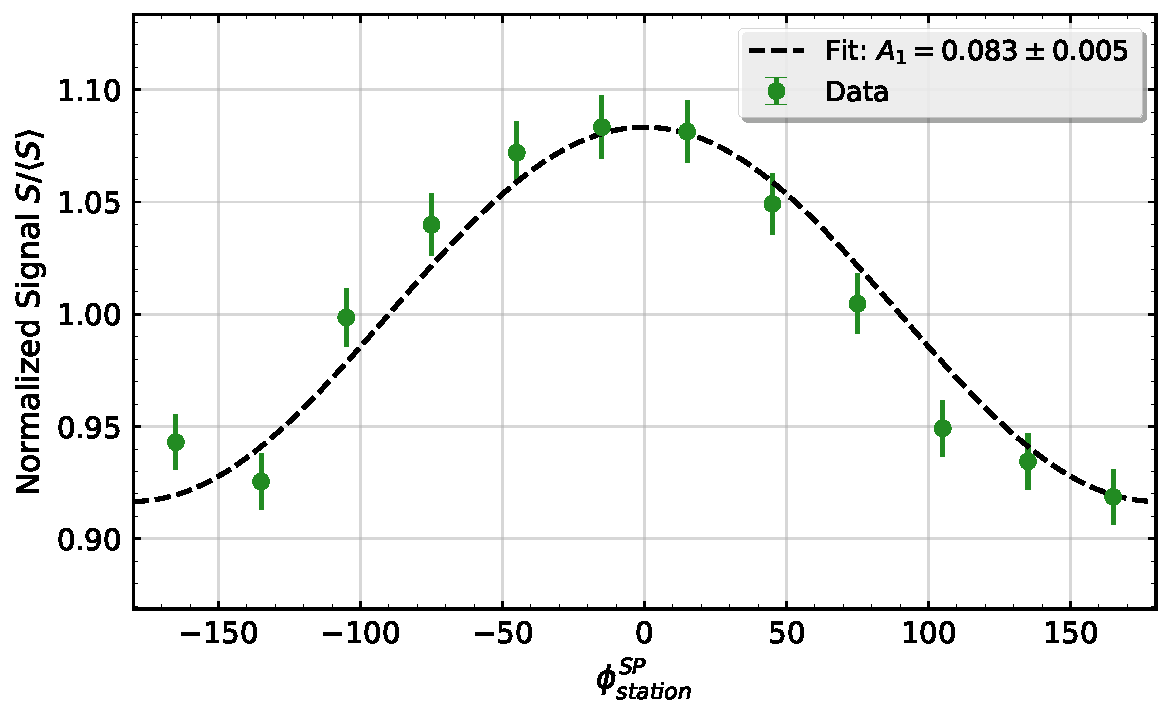
\includegraphics[width=1\textwidth]{Ajuste_UMD_MC_Bin9.pdf}
    \caption{Example of the first-order harmonic fit applied to the normalised MC muon density ($N_\mu^{\mathrm{MC}}$) in the Dense Ring topology ($r = 450$~m). The data corresponds to a representative highly inclined zenith bin. The signal exhibits a clear early excess ($\phi = 0^\circ$) and late deficit ($\phi = \pm 180^\circ$), yielding an asymmetry amplitude of $A_1 = 0.083 \pm 0.005$.}
    \label{fig:example_fit}
\end{figure}

For high inclinations ($\theta \gtrsim 50^{\circ}$), the atmospheric slant depth grows rapidly ($\propto \sec\theta$). The EM component is largely absorbed before reaching the ground, and the SD signal becomes progressively muon-dominated. In this regime the SD amplitude drops sharply, reflecting both the reduced EM contribution and the growing weight of the kinematic divergence acting on the low-energy muons that dominate the SD.

The UMD, which is by construction insensitive to the EM component, exhibits a smooth, monotonically increasing positive asymmetry that for higher inclinations  shows a slight magnitude decrease, but less significant than the SD. Because the soil overburden removes most of Population~B while preserving Population~A, the UMD tracks the atmospheric attenuation of the collimated, high-energy muonic backbone of the shower without being affected by the electromagnetic depletion and kinematic divergence that suppresses heavily the SD amplitude at large zenith angles.

\begin{figure}[h]
\centering
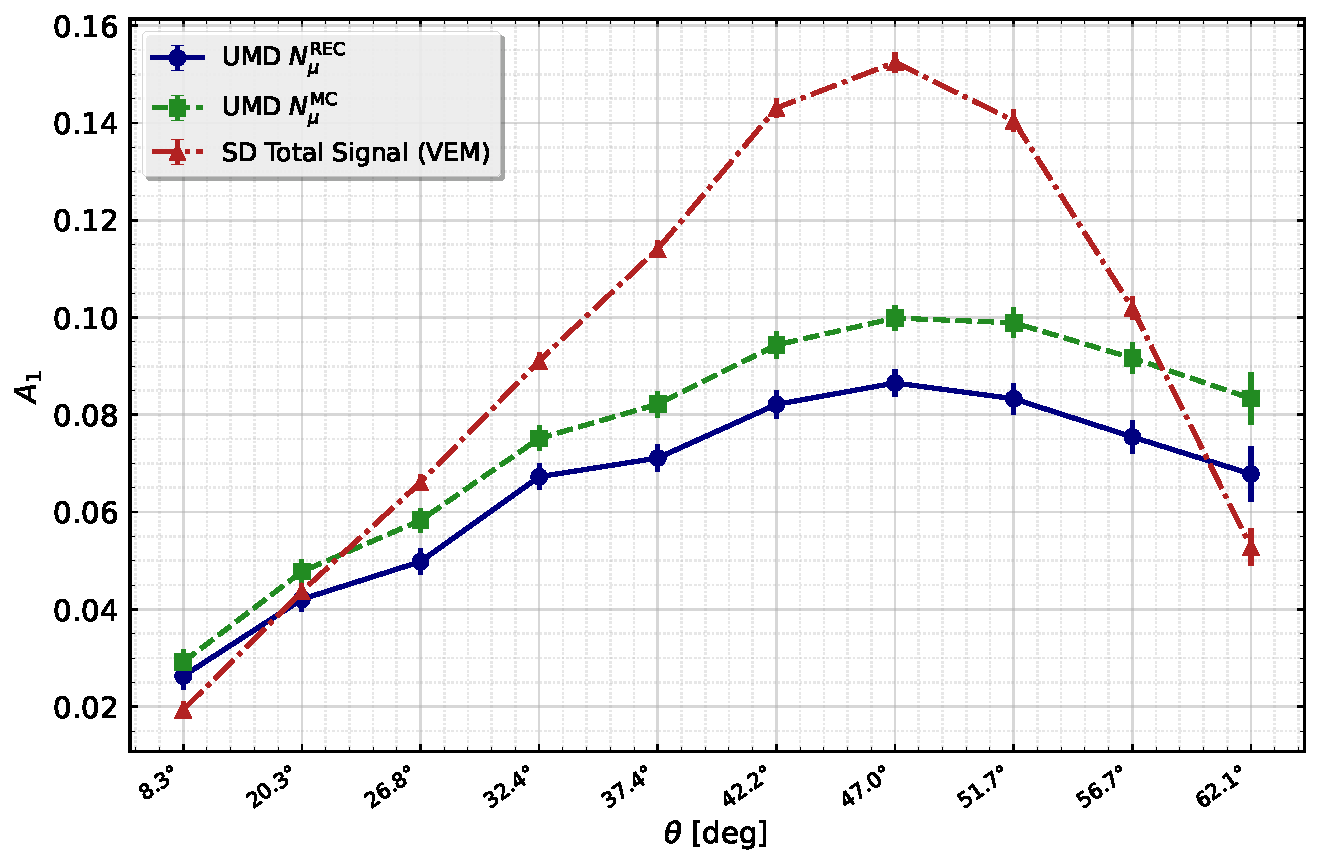
\includegraphics[width=1.0\textwidth]{Evolucion_Asimetria_vs_Theta.pdf}
\caption{Evolution of the first-harmonic amplitude $A_1$ as a function of the zenith angle $\theta$ in the Dense Ring topology ($r = 450$~m). The UMD is shown for reconstructed ($N_\mu^{\mathrm{REC}}$) and Monte Carlo true muons ($N_\mu^{\mathrm{MC}}$). The total SD signal in VEM units is also shown. A clear inversion of the hierarchy between the SD and the UMD is observed at high inclinations.}
\label{fig:evolucion_asym_vs_theta}
\end{figure}
\vspace{10cm}

\subsection{Radial Dynamics and the SD Muon Inversion}
\label{subsec:infill_results}

We now turn to the continuous radial spectrum provided by the 750~m array topology. Figure~\ref{fig:global_a1_umd_radial_zenith} shows the evolution of the UMD amplitude $A_1$, using the MC muons and coordinate system, as a function of the distance to the shower axis and the zenith angle. The amplitude increases both with radial distance, as expected from the growing difference in atmospheric slant depth between the early and late sides of the shower, and with inclination. For quasi-vertical showers ($\theta < 20^{\circ}$) the amplitude of the asymmetry is very close to zero.

The comparison of the UMD and the total SD signal in the 750~m array (Fig.~\ref{fig:umd_vs_sd_infill}) exposes a striking behavioural difference for the reference zenith bin $30^{\circ} \le \theta < 40^{\circ}$. The UMD amplitude grows smoothly towards positive values and plateaus at large $r$, in quantitative agreement with the expectation from atmospheric attenuation. In contrast, the total SD signal reaches a local maximum around $r \sim 700$~m and then drops sharply, crossing zero near $r \sim 1050$~m and becoming strongly negative at $r \gtrsim 1200$~m. This inversion is a genuine, geometric feature of the SD ground signal and merits an investigation into its physical origin.

\begin{figure}[h!]
    \centering
    \begin{subfigure}{1\textwidth}
        \centering
        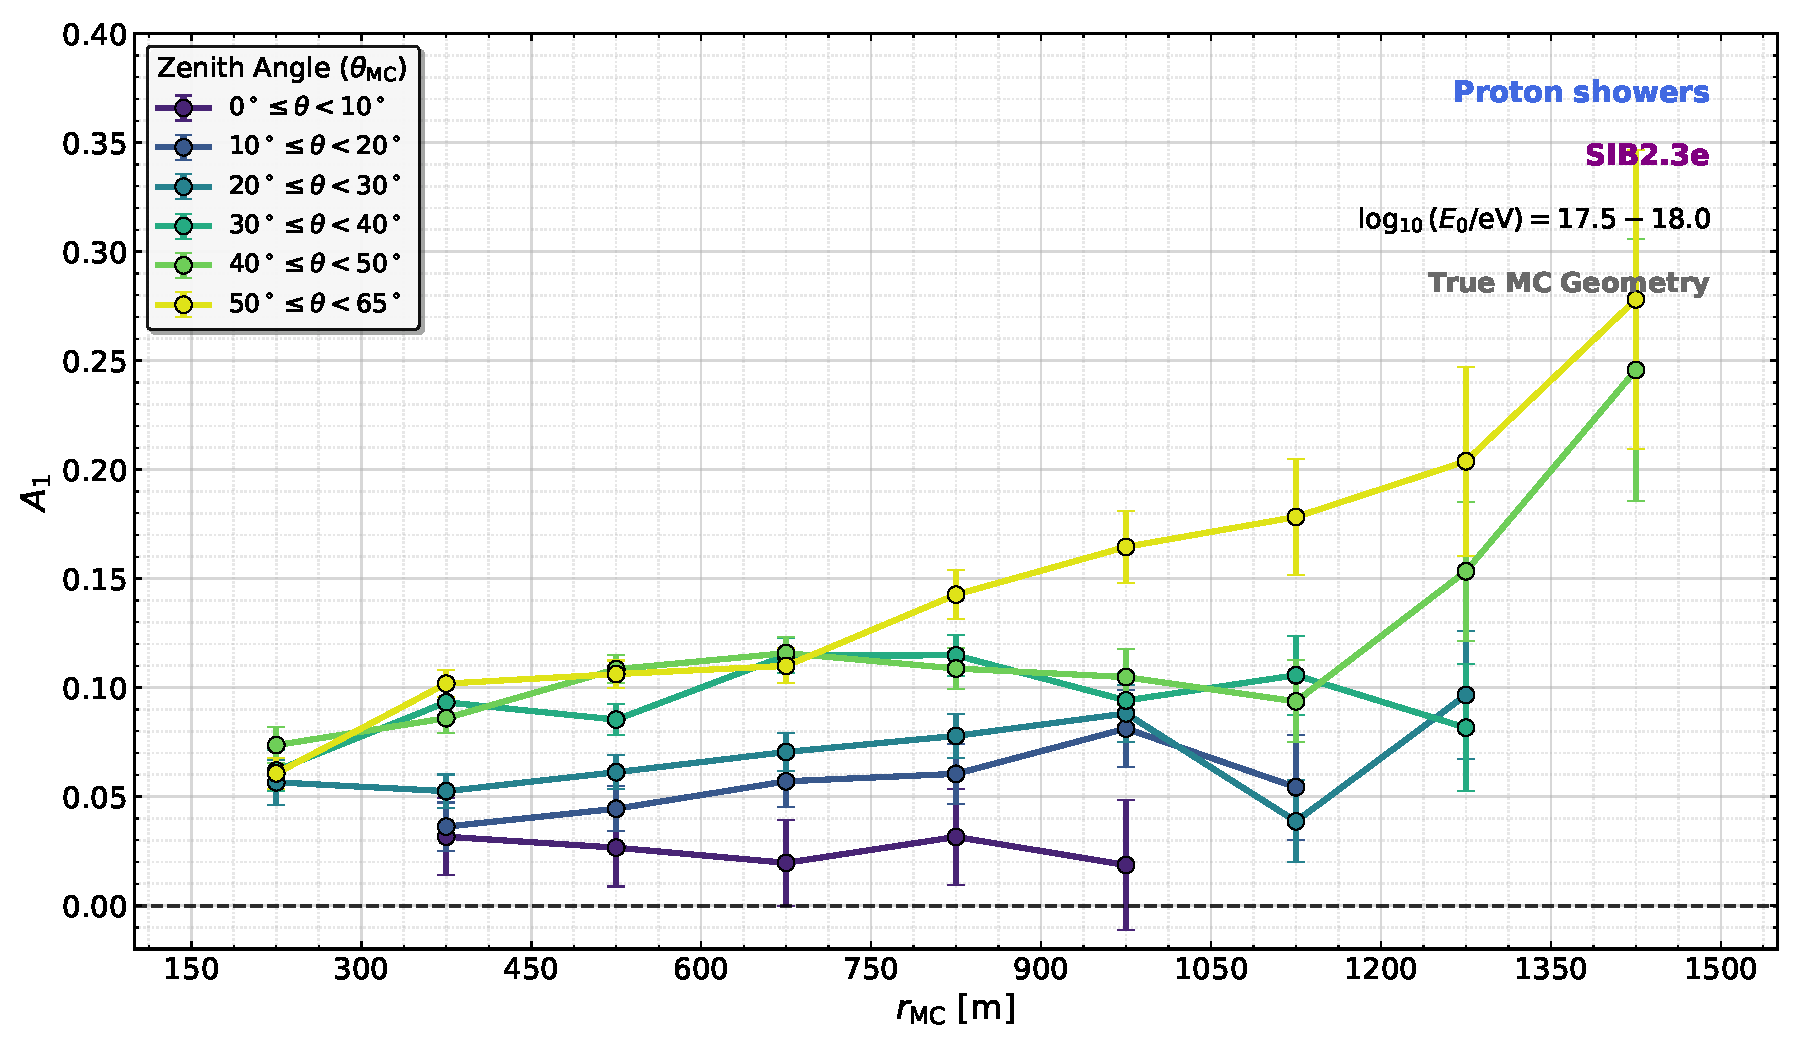
\includegraphics[width=0.94\textwidth]{Global_A1_vs_R_Theta_MC.pdf}
        \caption{}
        \label{fig:global_a1_umd_radial_zenith}
    \end{subfigure}
    \begin{subfigure}{1\textwidth}
        \centering
        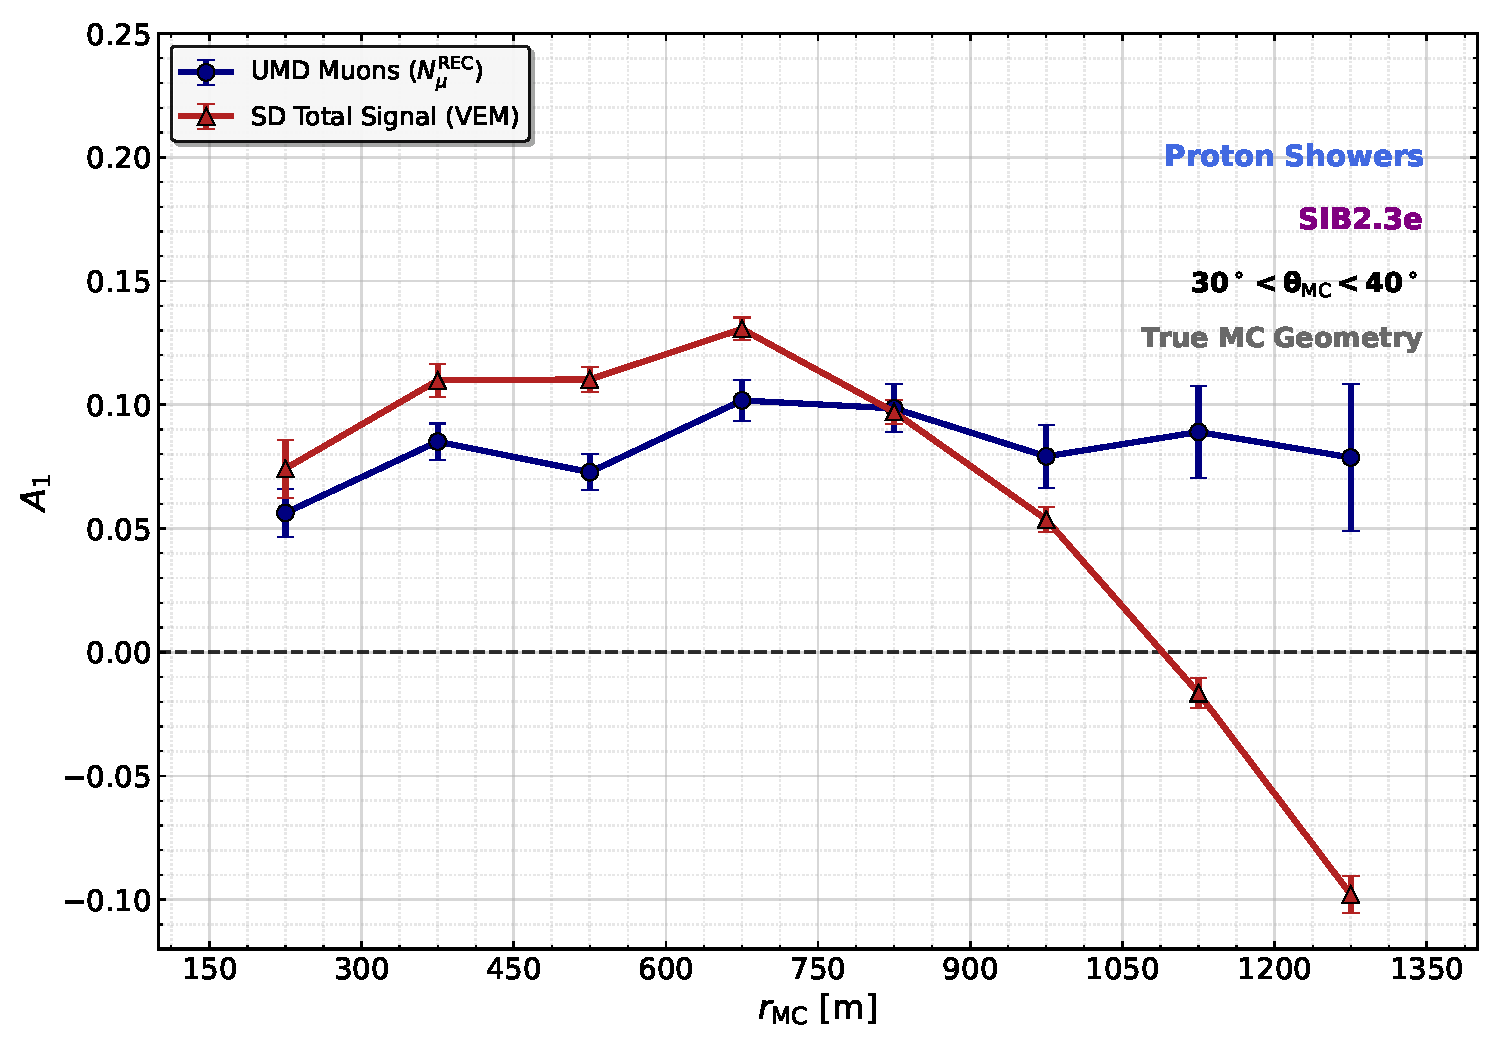
\includegraphics[width=0.94\textwidth]{UMD_vs_SD_Total_Asymmetry.pdf}
        \caption{}
        \label{fig:umd_vs_sd_infill}
    \end{subfigure}
    \caption{Top: Evolution of the UMD first-harmonic amplitude $A_1$ as a function of the distance to the shower axis across all evaluated zenith-angle bins. The amplitude grows monotonically with both radial distance and shower inclination. Bottom: Radial evolution of the first-harmonic amplitude $A_1$ comparing the pure muonic UMD signal ($N_\mu^{\mathrm{REC}}$) with the total SD signal (VEM) in the reference bin $30^{\circ} \le \theta < 40^{\circ}$. The UMD amplitude follows the attenuation-driven expectation, while the SD total signal undergoes a pronounced sign inversion in the far-core regime.}
\end{figure}
\vspace{10cm}

\subsection{Signal Dissection and the Kinematic Filter Mechanism}
\label{subsec:signal_dissection}

To pinpoint the physical origin of the SD inversion, we deconstruct the total VEM signal (shown in red) into its formative components at MC-truth level, the EM particle count reaching the detector ($N_{\mathrm{EM}}^{\mathrm{MC}}$) and the surface muon count ($N_{\mu, \mathrm{sup}}^{\mathrm{MC}}$). Figure~\ref{fig:sd_dissection} shows the radial evolution of $A_1$ for each of these components in the same zenith bin $30^{\circ} \le \theta < 40^{\circ}$.

The EM component displays a strongly positive asymmetry ($A_1 \sim 0.3$--$0.45$) across the whole radial range. Because EM particles are continuously produced and absorbed on short scales, their ground density is tightly coupled to the local longitudinal development of the cascade and is therefore a pure tracer of atmospheric attenuation.

The surface muons of the SD appear to be the driver of the inversion. Near the core they behave similarly to the UMD muons, but for $r \gtrsim 750$~m the amplitude decreases rapidly and crosses into the negative regime. Because the SD has low effective energy threshold for muons, the surface muon population is dominated by the low-momentum, highly divergent Population~B muons discussed in Sec.~\ref{subsec:divergence}. As those muons are precisely the ones for which the kinematic divergence term of Eq.~\eqref{eq:kinematic_divergence} is maximal, their compression onto the late region eventually overcomes the positive contribution of atmospheric attenuation and geometric effect, forcing $A_1 < 0$. The total SD signal inherits this sign inversion beyond $r \sim 1$~km. The proposed hypothesis for this behaviour is that at larger radii and higher zenith angles, the EM component is heavily depleted. Consequently, even though the EM asymmetry amplitude remains large, its relative contribution to the total signal becomes negligible. As the total signal becomes dominated by the muonic component—which carries a negative asymmetry due to kinematic divergence—the global SD asymmetry inverts.

\begin{figure}[h]
\centering
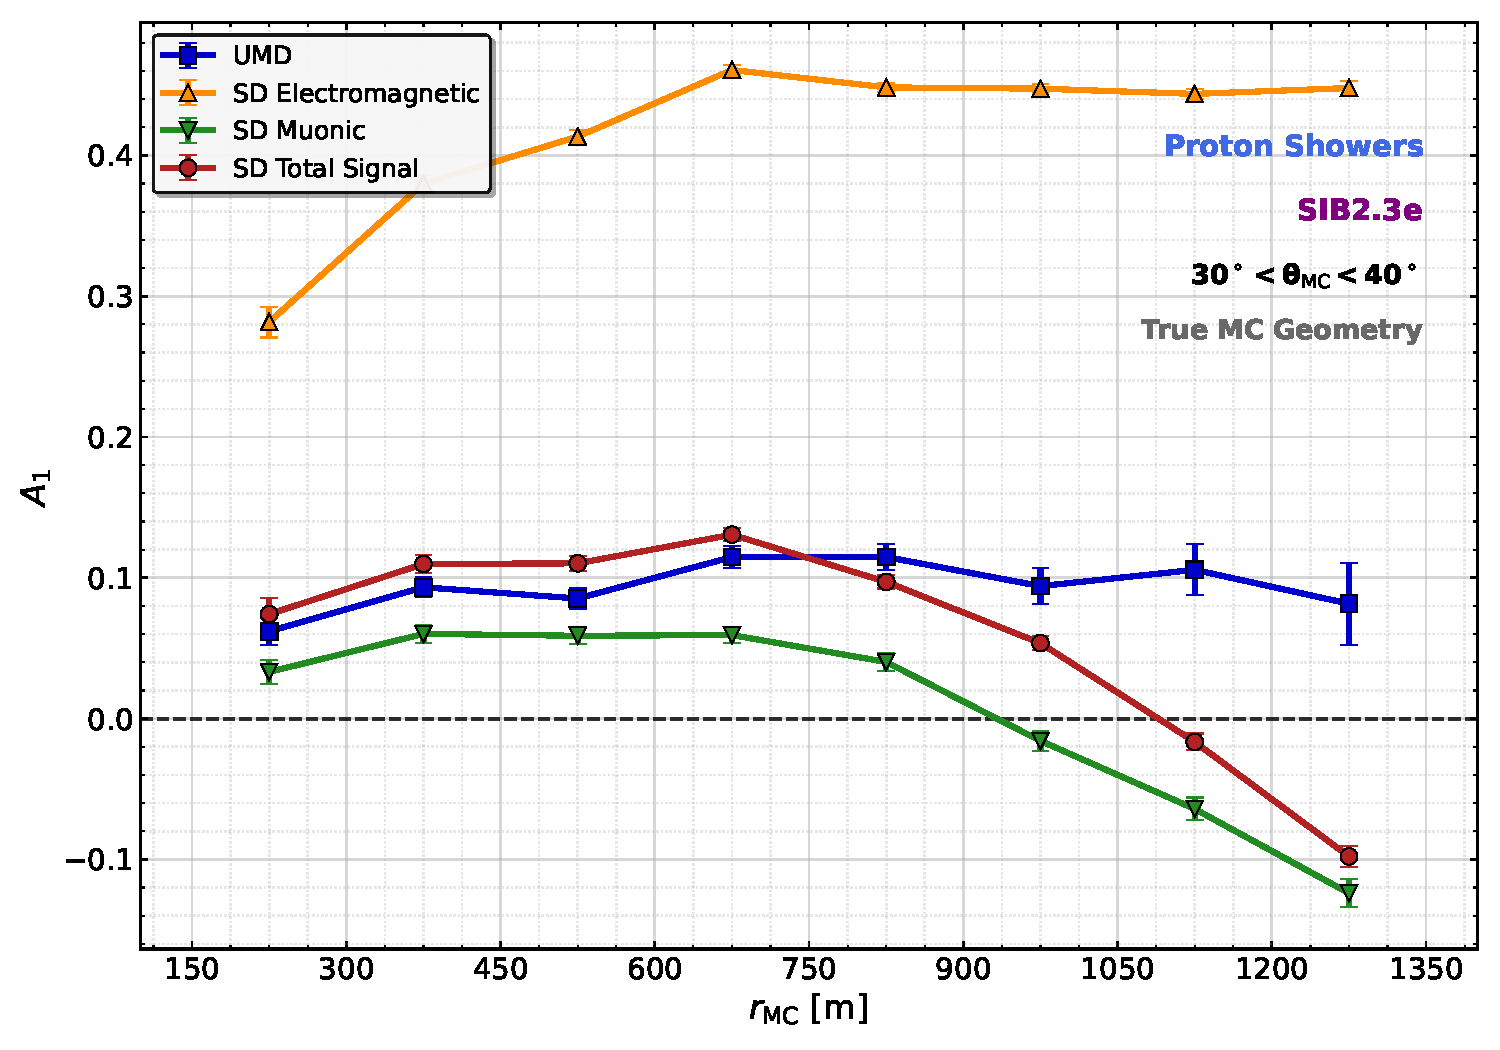
\includegraphics[width=1.0\textwidth]{SD_Desglose_Componentes_vs_UMD.pdf}
\caption{Deconstruction of the azimuthal asymmetry of the ground-level components compared with the UMD response in the reference bin $30^{\circ} \le \theta < 40^{\circ}$. The SD EM component shows a strongly positive attenuation asymmetry. The surface muons of the SD drive a negative geometric inversion at large radial distances. }
\label{fig:sd_dissection}
\end{figure}

The direct comparison with the UMD provides an empirical validation of this kinematic picture. The approximately $\sim 540~\mathrm{g/cm^{2}}$ soil overburden of the UMD acts as a strict kinematic filter that removes muons with $E_\mu \lesssim 1 ~\mathrm{GeV}/\cos\theta$ at ground level, precisely the Population~B muons responsible for the kinematic divergence term.

Table~\ref{tab:a1_summary} highlights this quantitative stability. With no kinematic effect, attenuation recovers full dominance and the UMD registers the robust, positive asymmetry intrinsic to the longitudinal development of the EAS.

\begin{table}[h]
\centering
\caption{Summary of azimuthal asymmetry amplitudes ($A_1$) for $\theta \in [30^\circ, 40^\circ]$ at selected shower-plane radii. Statistical fit uncertainties are typically $\le 0.02$.}
\label{tab:a1_summary}
\begin{tabular}{l c c c}
\toprule
\textbf{Observable} & \textbf{$r = 450$~m} & \textbf{$r = 800$~m} & \textbf{$r = 1200$~m} \\
\midrule
SD-EM (MC) & $+0.40$ & $+0.45$ & $+0.44$ \\
SD-Muon (MC) & $+0.05$ & $+0.04$ & $-0.10$ \\
SD Total (VEM) & $+0.11$ & $+0.09$ & $-0.08$ \\
UMD $N_\mu^{\mathrm{MC}}$ & $+0.10$ & $+0.12$ & $+0.11$ \\
\bottomrule
\end{tabular}
\end{table}

\newpage

\section{Conclusions}
\label{sec:conclusions}

We have revisited the phenomenology of the early--late azimuthal asymmetry of the muon density in extensive air showers and, for the first time, extended the analysis to the Underground Muon Detector of the AMIGA enhancement. Using the transport model of Caz\'on et al.~\cite{Cazon2012} and the geometric decomposition of Bertou and Billoir~\cite{GAP2000_017}, we have shown that the first-harmonic amplitude $A_1$ is determined by the competition between two opposing effects: a positive contribution from atmospheric attenuation and geometric effect and a negative contribution from the kinematic projection of low-energy, highly divergent muons.

At the level of the Surface Detector, this competition manifests itself in the pronounced sign inversion of $A_1$ observed in the far-core regime, reaching $A_1 \sim -0.08$ at $1200$~m for the total signal and $A_1 \sim -0.10$ for the pure SD surface muons. The deconstruction of the SD signal demonstrates that the inversion is entirely driven by the divergent muonic component (Population~B), whose contribution to the geometric term overwhelms the positive attenuation asymmetry of the EM component at large radial distances.

The Underground Muon Detector overcomes this limitation. The $2.3$~m soil overburden operates not merely as an EM absorber but, crucially, as an effective kinematic filter that suppresses Population~B and isolates the collimated high-energy backbone of the shower. In this regime, the exponential term of Eq.~\eqref{eq:kinematic_divergence} collapses to zero, so kinematic divergence effect no longer favours the late region. The UMD amplitude exhibits a smooth, positive and monotonic behaviour, reaching $A_1 \sim 0.11$ at $1200$~m, in quantitative agreement with the attenuation-only expectation.

These results establish the UMD as a phenomenologically cleaner instrument for the study of azimuthal asymmetries of the muonic component of ultra-high-energy air showers. The ability to decouple the muonic attenuation asymmetry from both EM contamination and geometric inversion opens the door to its exploitation as an independent probe of the longitudinal development of the cascade and, ultimately, of the primary mass composition. Extending the present analysis to quantify the residual geomagnetic contribution, assessing systematic model variances across \texttt{EPOS\,LHC-R} and \texttt{QGSJet-III.01}, comparing between other primaries and energy ranges and incorporating experimental smearing to confront the simulated response with AugerPrime data are natural next steps and will be the subject of forthcoming work.

\newpage
\bibliographystyle{unsrt}
\bibliography{bibliografia}

\end{document}